% Options for packages loaded elsewhere
% Options for packages loaded elsewhere
\PassOptionsToPackage{unicode}{hyperref}
\PassOptionsToPackage{hyphens}{url}
%
\documentclass[
  12pt,
  ignorenonframetext,
  aspectratio=169,
  brazilian,
  t]{beamer}
\newif\ifbibliography
\usepackage{pgfpages}
\setbeamertemplate{caption}[numbered]
\setbeamertemplate{caption label separator}{: }
\setbeamercolor{caption name}{fg=normal text.fg}
\beamertemplatenavigationsymbolsempty
% remove section numbering
\setbeamertemplate{part page}{
  \centering
  \begin{beamercolorbox}[sep=16pt,center]{part title}
    \usebeamerfont{part title}\insertpart\par
  \end{beamercolorbox}
}
\setbeamertemplate{section page}{
  \centering
  \begin{beamercolorbox}[sep=12pt,center]{section title}
    \usebeamerfont{section title}\insertsection\par
  \end{beamercolorbox}
}
\setbeamertemplate{subsection page}{
  \centering
  \begin{beamercolorbox}[sep=8pt,center]{subsection title}
    \usebeamerfont{subsection title}\insertsubsection\par
  \end{beamercolorbox}
}
% Prevent slide breaks in the middle of a paragraph
\widowpenalties 1 10000
\raggedbottom
\AtBeginPart{
  \frame{\partpage}
}
\AtBeginSection{
  \ifbibliography
  \else
    \frame{\sectionpage}
  \fi
}
\AtBeginSubsection{
  \frame{\subsectionpage}
}
\usepackage{iftex}
\ifPDFTeX
  \usepackage[T1]{fontenc}
  \usepackage[utf8]{inputenc}
  \usepackage{textcomp} % provide euro and other symbols
\else % if luatex or xetex
  \usepackage{unicode-math} % this also loads fontspec
  \defaultfontfeatures{Scale=MatchLowercase}
  \defaultfontfeatures[\rmfamily]{Ligatures=TeX,Scale=1}
\fi
\usepackage{lmodern}

\usetheme[]{default}
\usefonttheme{serif} % use mainfont rather than sansfont for slide text
\ifPDFTeX\else
  % xetex/luatex font selection
  \setmainfont[]{Segoe UI}
  \setsansfont[]{Segoe UI}
\fi
% Use upquote if available, for straight quotes in verbatim environments
\IfFileExists{upquote.sty}{\usepackage{upquote}}{}
\IfFileExists{microtype.sty}{% use microtype if available
  \usepackage[]{microtype}
  \UseMicrotypeSet[protrusion]{basicmath} % disable protrusion for tt fonts
}{}
\makeatletter
\@ifundefined{KOMAClassName}{% if non-KOMA class
  \IfFileExists{parskip.sty}{%
    \usepackage{parskip}
  }{% else
    \setlength{\parindent}{0pt}
    \setlength{\parskip}{6pt plus 2pt minus 1pt}}
}{% if KOMA class
  \KOMAoptions{parskip=half}}
\makeatother


\usepackage{longtable,booktabs,array}
\newcounter{none} % for unnumbered tables
\usepackage{calc} % for calculating minipage widths
\usepackage{caption}
% Make caption package work with longtable
\makeatletter
\def\fnum@table{\tablename~\thetable}
\makeatother
\usepackage{graphicx}
\makeatletter
\newsavebox\pandoc@box
\newcommand*\pandocbounded[1]{% scales image to fit in text height/width
  \sbox\pandoc@box{#1}%
  \Gscale@div\@tempa{\textheight}{\dimexpr\ht\pandoc@box+\dp\pandoc@box\relax}%
  \Gscale@div\@tempb{\linewidth}{\wd\pandoc@box}%
  \ifdim\@tempb\p@<\@tempa\p@\let\@tempa\@tempb\fi% select the smaller of both
  \ifdim\@tempa\p@<\p@\scalebox{\@tempa}{\usebox\pandoc@box}%
  \else\usebox{\pandoc@box}%
  \fi%
}
% Set default figure placement to htbp
\def\fps@figure{htbp}
\makeatother



\ifLuaTeX
\usepackage[bidi=basic,shorthands=off]{babel}
\else
\usepackage[bidi=default,shorthands=off]{babel}
\fi
\ifPDFTeX
\else
\babelfont{rm}[]{Segoe UI}
\fi
\ifLuaTeX
  \usepackage{selnolig} % disable illegal ligatures
\fi


\setlength{\emergencystretch}{3em} % prevent overfull lines

\providecommand{\tightlist}{%
  \setlength{\itemsep}{0pt}\setlength{\parskip}{0pt}}



 


% Identidade visual da apresentacao: azul-escuro, branco e detalhe coral.
\geometry{paperwidth=240mm,paperheight=135mm}
\setkeys{Gin}{keepaspectratio}
\definecolor{azulescuro}{HTML}{18324B}
\definecolor{azul}{HTML}{4477AA}
\definecolor{coral}{HTML}{EE6677}
\definecolor{cinzamedio}{HTML}{65727E}
\definecolor{cinzaclaro}{HTML}{EEF2F5}
\definecolor{textocorpo}{HTML}{25313C}
\definecolor{azulclaro}{HTML}{DCE6EE}
\usepackage{colortbl}
\setbeamercolor{normal text}{fg=textocorpo,bg=white}
\setbeamercolor{structure}{fg=azul}
\setbeamercolor{frametitle}{fg=azulescuro,bg=white}
\setbeamercolor{title}{fg=white}
\setbeamercolor{subtitle}{fg=azulclaro}
\setbeamerfont{title}{size=\fontsize{30}{35}\selectfont,series=\bfseries}
\setbeamerfont{subtitle}{size=\fontsize{16}{22}\selectfont}
\setbeamerfont{frametitle}{size=\fontsize{19}{23}\selectfont,series=\bfseries}
\setbeamersize{text margin left=11mm,text margin right=11mm}

% Corpo maior e entrelinha explicita, inclusive nas listas aninhadas.
\renewcommand{\normalsize}{\fontsize{13.5}{18.5}\selectfont}
\setbeamerfont{itemize/enumerate body}{size=\normalsize}
\setbeamerfont{itemize/enumerate subbody}{size=\normalsize}
\setbeamerfont{itemize/enumerate subsubbody}{size=\normalsize}
\setbeamertemplate{itemize/enumerate body begin}{\setlength{\itemsep}{5pt}\setlength{\parsep}{0pt}}
\setbeamertemplate{itemize/enumerate subbody begin}{\setlength{\itemsep}{3pt}\setlength{\parsep}{0pt}}
\setbeamertemplate{itemize item}{\small\textbullet}
\setbeamertemplate{itemize subitem}{\scriptsize\textbullet}
\setbeamertemplate{navigation symbols}{}
\setlength{\parskip}{6pt}
\setlength{\tabcolsep}{6pt}
\renewcommand{\tightlist}{\setlength{\itemsep}{4pt}\setlength{\parskip}{0pt}\setlength{\parsep}{0pt}}

% As paginas plain sao reservadas as aberturas das secoes.
\makeatletter
\setbeamertemplate{background canvas}{%
  \ifnum\c@framenumber=1\relax
    \color{azulescuro}\rule{\paperwidth}{\paperheight}%
  \else
    \ifbeamer@plainframe
      \color{azulescuro}\rule{\paperwidth}{\paperheight}%
    \else
      \color{white}\rule{\paperwidth}{\paperheight}%
    \fi
  \fi}
\makeatother

\setbeamertemplate{footline}{%
  \ifnum\value{framenumber}>1\relax
    \hfill{\color{cinzamedio}\fontsize{8}{10}\selectfont
    \insertframenumber\,/\,\inserttotalframenumber}\hspace{11mm}\vspace{3mm}%
  \fi}
\setbeamertemplate{frametitle}{%
  \vspace{3mm}\insertframetitle\par
  \vspace{1mm}{\color{azul}\hrule height 0.6pt}\vspace{3mm}}
\setbeamertemplate{caption}{\raggedright\insertcaption\par}

\newcommand{\SubtituloAbertura}[1]{%
  \noindent{\color{coral}\vrule width 2pt height 20pt depth 5pt}\hspace{5mm}%
  \begin{minipage}[c]{0.84\textwidth}
    \raggedright\color{azulclaro}\fontsize{16}{22}\selectfont #1
  \end{minipage}\par}
\setbeamertemplate{title page}{%
  \vspace*{26mm}
  \hspace*{7mm}\begin{minipage}{0.90\textwidth}
    \raggedright{\usebeamerfont{title}\color{white}\parbox{155mm}{\raggedright\inserttitle}\par}
    \vspace{10mm}
    \SubtituloAbertura{\insertsubtitle}
  \end{minipage}}
\newcommand{\AberturaSecao}[2]{%
  \vspace*{34mm}
  \hspace*{7mm}\begin{minipage}{0.90\textwidth}
    \raggedright{\color{white}\fontsize{32}{38}\selectfont\bfseries #1\par}
    \vspace{9mm}
    \SubtituloAbertura{#2}
  \end{minipage}}
\newcommand{\DescricaoIndicador}[1]{%
  {\color{azul}\fontsize{17}{23}\selectfont\bfseries #1\par}\vspace{4mm}}
\newcommand{\Rotulo}[1]{%
  \par\addvspace{7pt}{\color{azul}\bfseries #1\par}\nobreak\vspace{2pt}}
\newcommand{\TituloGrafico}[1]{{\fontsize{17.5}{21}\selectfont #1}}
\makeatletter
\@ifpackageloaded{caption}{}{\usepackage{caption}}
\AtBeginDocument{%
\ifdefined\contentsname
  \renewcommand*\contentsname{Índice}
\else
  \newcommand\contentsname{Índice}
\fi
\ifdefined\listfigurename
  \renewcommand*\listfigurename{Lista de Figuras}
\else
  \newcommand\listfigurename{Lista de Figuras}
\fi
\ifdefined\listtablename
  \renewcommand*\listtablename{Lista de Tabelas}
\else
  \newcommand\listtablename{Lista de Tabelas}
\fi
\ifdefined\figurename
  \renewcommand*\figurename{Figura}
\else
  \newcommand\figurename{Figura}
\fi
\ifdefined\tablename
  \renewcommand*\tablename{Tabela}
\else
  \newcommand\tablename{Tabela}
\fi
}
\@ifpackageloaded{float}{}{\usepackage{float}}
\floatstyle{ruled}
\@ifundefined{c@chapter}{\newfloat{codelisting}{h}{lop}}{\newfloat{codelisting}{h}{lop}[chapter]}
\floatname{codelisting}{Listagem}
\newcommand*\listoflistings{\listof{codelisting}{Lista de Listagens}}
\makeatother
\makeatletter
\makeatother
\makeatletter
\@ifpackageloaded{caption}{}{\usepackage{caption}}
\@ifpackageloaded{subcaption}{}{\usepackage{subcaption}}
\makeatother

\usepackage{bookmark}
\IfFileExists{xurl.sty}{\usepackage{xurl}}{} % add URL line breaks if available
\urlstyle{same}
% fallback for those not using the hyperref driver hyperxmp:
\makeatletter
\@ifundefined{xmpquote}{\newcommand{\xmpquote}[1]{#1}}{}
\makeatother
\hypersetup{
  pdftitle={Monitoramento da educação superior a distância},
  pdflang={pt-BR},
  hidelinks,
  pdfcreator={LaTeX via pandoc}}


\title{\texorpdfstring{Monitoramento da educação superior a
distância}{Monitoramento da educação superior a distância}}
\subtitle{\texorpdfstring{Resultados disponíveis e estrutura das fichas
das dimensões
A--H}{Resultados disponíveis e estrutura das fichas das dimensões A--H}}
\author{}
\date{}

\begin{document}
\frame{\titlepage}


\begin{frame}[plain]{}
\protect\phantomsection\label{introduuxe7uxe3o}
\AberturaSecao{Introdução}{Dimensões, fontes e principais escolhas de processamento}
\end{frame}

\begin{frame}{Dimensões}
\protect\phantomsection\label{dimensuxf5es}
\begin{columns}[T]
\begin{column}{0.47\linewidth}
\Rotulo{A. Rede institucional e oferta}

Quem oferta e como o sistema está organizado? \textbf{\emph{5
indicadores}}.

\Rotulo{B. Padrão de crescimento do setor}

Com qual velocidade o sistema cresceu? Onde surgiram as novas
matrículas? \textbf{\emph{3 indicadores}}.

\Rotulo{C. Dinâmica do mercado: extinções, fusões e crescimento}

O que o e-MEC revela sobre o ensino superior entre 2010 e 2024? \emph{1
indicador}.

\Rotulo{D. Quem são os proprietários das mantenedoras das IES no Brasil?}

Análise a partir dos dados abertos da Receita Federal. \emph{1
indicador}.
\end{column}

\begin{column}{0.47\linewidth}
\Rotulo{E. Acesso e matrícula}

Quem chega ao ensino superior e como? \emph{2 indicadores}.

\Rotulo{F. Fluxo acadêmico e conclusão}

Quem permanece e se forma? \emph{3 indicadores}.

\Rotulo{G. Corpo docente}

Quem ensina e em que condições? \textbf{\emph{4 indicadores}}.

\Rotulo{H. Equidade e Inclusão}

Quem fica de fora e por quê? \emph{4 indicadores}.
\end{column}
\end{columns}
\end{frame}

\begin{frame}{Dados e métodos}
\protect\phantomsection\label{dados-e-muxe9todos}
\Rotulo{Fontes}

Microdados públicos do Censo do Ensino Superior, 2010-2024.

\Rotulo{Filtros}

\textbf{1.} Exclusão de cursos EaD ofertados no exterior.

\textbf{2.} Exclusão de cursos sequenciais de formação específica.

\textbf{3.} Exclusão de IES sem cursos válidos.

\Rotulo{Harmonização de variáveis}

\textbf{1.} Código de mantenedora

\textbf{2.} Categoria administrativa.

\textbf{3.} Organização acadêmica.

\textbf{4.} Faixa de tamanho da mantenedora segundo o ranking anual de
matrículas.
\end{frame}

\begin{frame}{Categoria administrativa}
\protect\phantomsection\label{categoria-administrativa}
\Rotulo{Problemas}

\textbf{1.} Mudanças de categoria administrativa entre IES que
permaneceram ativas em anos consecutivos.

\begin{itemize}
\tightlist
\item
  399 das 3.676 IES, ou \textbf{11\%}.
\end{itemize}

\textbf{2.} Mantenedoras com IES pertencentes a diferentes categorias
administrativas em um mesmo ano.

\begin{itemize}
\tightlist
\item
  36 das 2,788 mantenedoras, ou \textbf{1\%}.
\end{itemize}

\vfill

\Rotulo{Harmonização}

\textbf{1.} Corrige mudanças anuais em IES públicas.

\begin{itemize}
\tightlist
\item
  IES federais ou estaduais reclassificadas conforme o valor modal das
  cinco aparições mais recentes;
\item
  Combinações mantenedora-IES municipais reclassificadas conforme o nome
  e a moda.
\end{itemize}

\textbf{2.} Corrige multiplicidade de categorias administrativas para
uma mantenedora em um mesmo ano.

\begin{itemize}
\tightlist
\item
  Reclassifica como públicas as mantenedoras com alguma IES pública;
  como ``com fins lucrativos'' as mantenedoras cujo nome denota empresas
  que visam o lucro; e agrega ``sem fins lucrativos'' e ``especial''.
\end{itemize}
\end{frame}

\begin{frame}[plain]{}
\protect\phantomsection\label{dimensuxe3o-a}
\AberturaSecao{Dimensão A}{Rede institucional e oferta}
\end{frame}

\begin{frame}{A.1}
\protect\phantomsection\label{a.1}
\DescricaoIndicador{Número e distribuição de IES e mantenedoras por categoria administrativa e organização acadêmica entre 2010 e 2024}

\Rotulo{Séries}

\begin{itemize}
\tightlist
\item
  IES:

  \begin{itemize}
  \tightlist
  \item
    Total
  \item
    Categoria administrativa
  \item
    Organização acadêmica
  \item
    Categoria administrativa + organização acadêmica
  \end{itemize}
\item
  Mantenedoras:

  \begin{itemize}
  \tightlist
  \item
    Total
  \item
    Categoria administrativa
  \end{itemize}
\end{itemize}
\end{frame}

\begin{frame}{\TituloGrafico{A.1 --- Quantidade de mantenedoras e de IES}}
\protect\phantomsection\label{a.1-quantidade-de-mantenedoras-e-de-ies}
\begin{center}
\includegraphics[width=218mm,height=98mm,keepaspectratio]{../../relatorio/figuras/figura01.png}
\end{center}

\vfill
\begingroup
\fontsize{8}{10}\selectfont\color{cinzamedio}

Fonte: elaboração própria com base no Censo da Educação Superior.

\endgroup
\end{frame}

\begin{frame}{\TituloGrafico{A.1 --- Quantidade de IES por categoria administrativa}}
\protect\phantomsection\label{a.1-quantidade-de-ies-por-categoria-administrativa}
\begin{center}
\includegraphics[width=218mm,height=98mm,keepaspectratio]{../../relatorio/figuras/figura02.png}
\end{center}

\vfill
\begingroup
\fontsize{8}{10}\selectfont\color{cinzamedio}

Fonte: elaboração própria com base no Censo da Educação Superior.

\endgroup
\end{frame}

\begin{frame}{A.1 --- Principais conclusões}
\protect\phantomsection\label{a.1-principais-conclusuxf5es}
\Rotulo{Expansão modesta no agregado}

\begin{itemize}
\tightlist
\item
  Entre 2010 e 2024, o total de IES cresceu \textbf{8\%}, enquanto o
  número de mantenedoras aumentou apenas \textbf{2\%}.
\end{itemize}

\Rotulo{Mudanças expressivas de composição}

\begin{itemize}
\tightlist
\item
  O número de IES ligadas a mantenedoras com fins lucrativos aumentou
  quase \textbf{60\%}; entre as sem fins lucrativos, caiu \textbf{36\%};
\item
  A mudança acelerou entre 2016 e 2019, impulsionado pela
  reclassificação de IES existentes;
\item
  Ou seja, mudança não representa apenas abertura e fechamento de
  instituições.
\end{itemize}
\end{frame}

\begin{frame}{A.2}
\protect\phantomsection\label{a.2}
\DescricaoIndicador{Número de vagas oferecidas e taxa de ocupação por modalidade (presencial e ensino a distância) entre 2010 e 2024}

\Rotulo{Séries}

\begin{itemize}
\tightlist
\item
  Ingressantes, vagas e taxa de ingressantes por 100 vagas:

  \begin{itemize}
  \tightlist
  \item
    Total
  \item
    Modalidade de ensino
  \end{itemize}
\end{itemize}
\end{frame}

\begin{frame}{\TituloGrafico{A.2 --- Quantidade de vagas por modalidade de ensino}}
\protect\phantomsection\label{a.2-quantidade-de-vagas-por-modalidade-de-ensino}
\begin{center}
\includegraphics[width=218mm,height=98mm,keepaspectratio]{../../relatorio/figuras/figura03.png}
\end{center}

\vfill
\begingroup
\fontsize{8}{10}\selectfont\color{cinzamedio}

Fonte: elaboração própria com base no Censo da Educação Superior. Taxa
de ocupação: ingressantes por 100 vagas oferecidas.

\endgroup
\end{frame}

\begin{frame}{\TituloGrafico{A.2 --- Taxa de ocupação das vagas por modalidade de ensino}}
\protect\phantomsection\label{a.2-taxa-de-ocupauxe7uxe3o-das-vagas-por-modalidade-de-ensino}
\begin{center}
\includegraphics[width=218mm,height=98mm,keepaspectratio]{../../relatorio/figuras/figura04.png}
\end{center}

\vfill
\begingroup
\fontsize{8}{10}\selectfont\color{cinzamedio}

Fonte: elaboração própria com base no Censo da Educação Superior. Taxa
de ocupação: ingressantes por 100 vagas oferecidas.

\endgroup
\end{frame}

\begin{frame}{A.2 --- Principais conclusões}
\protect\phantomsection\label{a.2-principais-conclusuxf5es}
\Rotulo{Forte expansão da oferta}

\begin{itemize}
\tightlist
\item
  A oferta de vagas multiplicou-se por cinco entre 2010 e 2024; cerca de
  \textbf{90\% da expansão} veio da EaD;
\item
  Desaceleração da expansão após 2021, com retração em 2024;
\item
  Ritmo da mudança na composição das vagas também arrefeceu.
\end{itemize}

\Rotulo{Oferta avançou mais rapidamente do que a demanda}

\begin{itemize}
\tightlist
\item
  A taxa de ocupação total caiu de \textbf{46\% para 21\%} entre 2010 e
  2024. Em 2024, alcançou 33\% no presencial e 18\% na EaD;
\item
  Estabilização da oferta de vagas nos últimos anos coincidiu com
  recuperação nas taxas de ocupação, sobretudo para o ensino presencial.
\end{itemize}
\end{frame}

\begin{frame}{A.3 *}
\protect\phantomsection\label{a.3}
\DescricaoIndicador{Distribuição de ingressantes e matrículas por modalidade (presencial e EaD) e turno entre 2010 e 2024}

\Rotulo{Séries}

\begin{itemize}
\tightlist
\item
  Ingressantes e matrículas:

  \begin{itemize}
  \tightlist
  \item
    Total
  \item
    Modalidade de ensino
  \item
    Turno de ensino
  \end{itemize}
\end{itemize}
\end{frame}

\begin{frame}{\TituloGrafico{A.3 --- Quantidade de ingressantes por modalidade e turno}}
\protect\phantomsection\label{a.3-quantidade-de-ingressantes-por-modalidade-e-turno}
\begin{center}
\includegraphics[width=218mm,height=98mm,keepaspectratio]{../../relatorio/figuras/figura05.png}
\end{center}

\vfill
\begingroup
\fontsize{8}{10}\selectfont\color{cinzamedio}

Fonte: elaboração própria com base no Censo da Educação Superior.

\endgroup
\end{frame}

\begin{frame}{\TituloGrafico{A.3 --- Quantidade de matrículas por modalidade e turno}}
\protect\phantomsection\label{a.3-quantidade-de-matruxedculas-por-modalidade-e-turno}
\begin{center}
\includegraphics[width=218mm,height=98mm,keepaspectratio]{../../relatorio/figuras/figura06.png}
\end{center}

\vfill
\begingroup
\fontsize{8}{10}\selectfont\color{cinzamedio}

Fonte: elaboração própria com base no Censo da Educação Superior.

\endgroup
\end{frame}

\begin{frame}{A.3 --- Principais conclusões}
\protect\phantomsection\label{a.3-principais-conclusuxf5es}
\Rotulo{Quantidade de ingressantes aumentou 130\%}

\begin{itemize}
\tightlist
\item
  Crescimento inteiramente provocado pelo EaD, que multiplicou por
  \textbf{nove};
\item
  EaD superou o presencial noturno em 2018 e, desde 2020, supera a soma
  do presencial noturno e do diurno. Em 2024, quase \textbf{67\%} dos
  ingressantes estavam no EaD;
\item
  Presencial noturno caiu \textbf{36\%} desde o pico em 2014; já o
  presencial diurno atingiu seu pico histórico em 2017, mas depois
  recuou \textbf{20\%}.
\end{itemize}

\Rotulo{Quantidade de matrículas aumentou 60\%}

\begin{itemize}
\tightlist
\item
  Mais uma vez, crescimento puxado por EaD, que ultrapassou
  \textbf{50\%} do total de matrículas em 2024;
\item
  Forte redução absoluta e relativa do ensino presencial noturno: no
  pico, em 2015, eram 4.1 milhões de matrículas, representando 51\% do
  total; em 2024, esse número caiu para 2.7 milhões (\textbf{-34\%}), o
  equivalente a apenas 27\% das matrículas.
\end{itemize}
\end{frame}

\begin{frame}{A.4 *}
\protect\phantomsection\label{a.4}
\DescricaoIndicador{Distribuição de ingressantes e matrículas por tamanho da mantenedora (presencial e EaD) entre 2010 e 2024}

\Rotulo{Séries}

\begin{itemize}
\tightlist
\item
  Ingressantes e matrículas:

  \begin{itemize}
  \tightlist
  \item
    Total
  \item
    Modalidade de ensino
  \item
    Tamanho de mantenedoras por número de matrículas
  \item
    Tamanho de mantenedoras por número de matrículas + Modalidade de
    ensino
  \end{itemize}
\end{itemize}
\end{frame}

\begin{frame}{\TituloGrafico{A.4 --- Quantidade de ingressantes por tamanho da mantenedora}}
\protect\phantomsection\label{a.4-quantidade-de-ingressantes-por-tamanho-da-mantenedora}
\begin{center}
\includegraphics[width=218mm,height=98mm,keepaspectratio]{../../relatorio/figuras/figura07.png}
\end{center}

\vfill
\begingroup
\fontsize{8}{10}\selectfont\color{cinzamedio}

Fonte: elaboração própria com base no Censo da Educação Superior. As
faixas são recalculadas anualmente.

\endgroup
\end{frame}

\begin{frame}{\TituloGrafico{A.4 --- Quantidade de matrículas por tamanho da mantenedora}}
\protect\phantomsection\label{a.4-quantidade-de-matruxedculas-por-tamanho-da-mantenedora}
\begin{center}
\includegraphics[width=218mm,height=98mm,keepaspectratio]{../../relatorio/figuras/figura08.png}
\end{center}

\vfill
\begingroup
\fontsize{8}{10}\selectfont\color{cinzamedio}

Fonte: elaboração própria com base no Censo da Educação Superior. As
faixas são recalculadas anualmente.

\endgroup
\end{frame}

\begin{frame}{A.4 --- Principais conclusões}
\protect\phantomsection\label{a.4-principais-conclusuxf5es}
\Rotulo{Ingressantes}

\begin{itemize}
\tightlist
\item
  As cinco maiores mantenedoras passaram de cerca de 375 mil
  ingressantes em 2010 para 1.9 milhões em 2024; com isso, sua
  participação subiu de \textbf{17\%} para \textbf{38\%};
\item
  A participação das 20 maiores mantenedoras aumentou de \textbf{29\%}
  para \textbf{57\%} dos ingressantes;
\item
  Leve recuo da participação das maiores mantenedoras em 2023 e 2024,
  depois do pico em 2022.
\end{itemize}

\Rotulo{Matrículas}

\begin{itemize}
\tightlist
\item
  As cinco maiores mantenedoras passaram de cerca de 800 mil matrículas
  em 2010 para 2.8 milhões em 2024, subindo de \textbf{13\%} para
  \textbf{27\%} do total;
\item
  A participação das 20 maiores aumentou de \textbf{26\% para 45\%}
  chegando a 4.6m de matrículas;
\item
  O pico histórico de concentração das matrículas foi em 2023, com recuo
  em 2024.
\end{itemize}

\Rotulo{Observação}

\begin{itemize}
\tightlist
\item
  Como o ranking muda a cada ano, a ficha mede concentração por faixa,
  não a trajetória de um conjunto fixo de grupos.
\end{itemize}
\end{frame}

\begin{frame}{A.5}
\protect\phantomsection\label{a.5}
\DescricaoIndicador{Distribuição de ingressantes e matrículas por área de conhecimento (CINE Brasil) e modalidade (presencial e ensino a distância) entre 2010 e 2024}

\Rotulo{Séries}

\begin{itemize}
\tightlist
\item
  Ingressantes e matrículas:

  \begin{itemize}
  \tightlist
  \item
    Total
  \item
    Área do conhecimento
  \item
    Modalidade de ensino
  \item
    Área do conhecimento + Modalidade de ensino
  \end{itemize}
\end{itemize}
\end{frame}

\begin{frame}{\TituloGrafico{A.5 --- Quantidade de ingressantes por área do conhecimento}}
\protect\phantomsection\label{a.5-quantidade-de-ingressantes-por-uxe1rea-do-conhecimento}
\begin{center}
\includegraphics[width=218mm,height=98mm,keepaspectratio]{../../relatorio/figuras/figura09.png}
\end{center}

\vfill
\begingroup
\fontsize{8}{10}\selectfont\color{cinzamedio}

Fonte: elaboração própria com base no Censo da Educação Superior.

\endgroup
\end{frame}

\begin{frame}{\TituloGrafico{A.5 --- Participação da EaD por área do conhecimento}}
\protect\phantomsection\label{a.5-participauxe7uxe3o-da-ead-por-uxe1rea-do-conhecimento}
\begin{center}
\includegraphics[width=218mm,height=98mm,keepaspectratio]{../../relatorio/figuras/figura10.png}
\end{center}

\vfill
\begingroup
\fontsize{8}{10}\selectfont\color{cinzamedio}

Fonte: elaboração própria com base no Censo da Educação Superior.

\endgroup
\end{frame}

\begin{frame}{A.5 --- Principais conclusões}
\protect\phantomsection\label{a.5-principais-conclusuxf5es}
\Rotulo{Expansão foi generalizada, porém com diferenças de intensidade e cronologia}

\begin{itemize}
\tightlist
\item
  Saúde e Bem-estar registrou o maior crescimento absoluto entre 2010 e
  2024, com acréscimo de cerca de \textbf{753 mil} ingressantes;
\item
  O sistema permaneceu concentrado em poucas áreas, apesar de alguma
  diversificação ao longo do período: as quatro principais áreas
  atraíram \textbf{82\%} dos ingressantes em 2010 e \textbf{77\%} em
  2024;
\item
  Concentração caiu devido ao forte crescimento de Computação e TIC e
  Serviços.
\end{itemize}

\Rotulo{EaD cresceu em todas as áreas, mas também com intensidade variável}

\begin{itemize}
\tightlist
\item
  Em 2010, a EaD era minoritária entre os ingressantes de todas as
  áreas; em 2024, já reunia a maioria dos ingressantes em \textbf{sete
  das onze áreas} analisadas.
\item
  A participação do EaD chegou a \textbf{87\% em Serviços} e
  \textbf{82\% em Educação}; também superou 70\% em Negócios, Artes e
  Humanidades e Computação e TIC.
\end{itemize}
\end{frame}

\begin{frame}[plain]{}
\protect\phantomsection\label{dimensuxe3o-b}
\AberturaSecao{Dimensão B}{Padrões de crescimento do setor}
\end{frame}

\begin{frame}{B.1 *}
\protect\phantomsection\label{b.1}
\DescricaoIndicador{Apropriação acumulada do saldo de ingressantes e matrículas por categoria administrativa, turno e modalidade (presencial e EaD) entre 2010 e 2024}

\Rotulo{Séries}

\begin{itemize}
\tightlist
\item
  Ingressantes e matrículas:

  \begin{itemize}
  \tightlist
  \item
    Total
  \item
    Categoria administrativa
  \item
    Modalidade de ensino
  \item
    Turno de ensino
  \item
    Categoria administrativa + Modalidade de ensino
  \item
    Categoria administrativa + Turno de ensino
  \end{itemize}
\end{itemize}
\end{frame}

\begin{frame}{\TituloGrafico{B.1 --- Variação de matrículas por categoria, modalidade e turno,
2010/2024}}
\protect\phantomsection\label{b.1-variauxe7uxe3o-de-matruxedculas-por-categoria-modalidade-e-turno-20102024}
\begin{center}\begingroup\fontsize{10.5}{12}\selectfont

\begin{tabular}{p{0.57\textwidth}rr}
\toprule
\rowcolor{azulescuro}
\textcolor{white}{\textbf{Grupos}} & \textcolor{white}{\textbf{Variação (milhares)}} & \textcolor{white}{\textbf{Contribuição (\%)}}\\
\midrule
\rowcolor{cinzaclaro}\textbf{Pública Federal} & 379 & 10\\
\hspace{1em}Educação a Distância & -13 & 0\\
\hspace{1em}Diurno & 258 & 7\\
\hspace{1em}Noturno & 134 & 3\\
\rowcolor{cinzaclaro}\textbf{Pública Estadual} & 66 & 2\\
\hspace{1em}Educação a Distância & 45 & 1\\
\hspace{1em}Diurno & 36 & 1\\
\hspace{1em}Noturno & -16 & 0\\
\rowcolor{cinzaclaro}\textbf{Pública Municipal} & -26 & -1\\
\hspace{1em}Educação a Distância & 2 & 0\\
\hspace{1em}Diurno & 4 & 0\\
\hspace{1em}Noturno & -32 & -1\\
\rowcolor{cinzaclaro}\textbf{Privada com fins lucrativos} & 4,357 & 113\\
\hspace{1em}Educação a Distância & 4,001 & 104\\
\hspace{1em}Diurno & 232 & 6\\
\hspace{1em}Noturno & 124 & 3\\
\rowcolor{cinzaclaro}\textbf{Privada sem fins lucrativos} & -931 & -24\\
\hspace{1em}Educação a Distância & 222 & 6\\
\hspace{1em}Diurno & -217 & -6\\
\hspace{1em}Noturno & -936 & -24\\
\rowcolor{cinzaclaro}\textbf{Total} & 3,845 & 100\\
\bottomrule
\end{tabular}
\endgroup\end{center}

\vfill
\begingroup
\fontsize{8}{10}\selectfont\color{cinzamedio}

Fonte: elaboração própria com base nos dados do Censo da Educação
Superior.

\endgroup
\end{frame}

\begin{frame}{B.1 --- Principais conclusões}
\protect\phantomsection\label{b.1-principais-conclusuxf5es}
\Rotulo{Profunda mudança de composição no ensino superior}

\begin{itemize}
\tightlist
\item
  O sistema ganhou cerca de \textbf{3.8 milhões de matrículas} entre
  2010 e 2024;
\item
  A combinação ``privada com fins lucrativos + EaD'' cresceu \textbf{4.0
  milhões}, valor superior ao saldo líquido de todo o sistema;
\item
  Ensino presencial noturno em IES privadas sem fins lucrativos diminuiu
  em \textbf{936 mil};
\item
  Maior crescimento do ensino presencial ocorreu nas públicas federais.
\end{itemize}
\end{frame}

\begin{frame}{B.2}
\protect\phantomsection\label{b.2}
\DescricaoIndicador{Apropriação acumulada do saldo de ingressantes e matrículas por área de conhecimento (CINE Brasil), categoria administrativa e modalidade (presencial e ensino a distância) entre 2010 e 2024}

\Rotulo{Séries}

\begin{itemize}
\tightlist
\item
  Ingressantes e matrículas:

  \begin{itemize}
  \tightlist
  \item
    Total
  \item
    Área do conhecimento
  \item
    Categoria administrativa
  \item
    Modalidade de ensino
  \item
    Turno de ensino
  \item
    Área do conhecimento + Modalidade de ensino
  \item
    Área do conhecimento + Turno de ensino
  \item
    Categoria administrativa + todas as combinações
  \end{itemize}
\end{itemize}
\end{frame}

\begin{frame}{\TituloGrafico{B.2 --- Variação de matrículas por área e modalidade}}
\protect\phantomsection\label{b.2-variauxe7uxe3o-de-matruxedculas-por-uxe1rea-e-modalidade}
\begin{center}
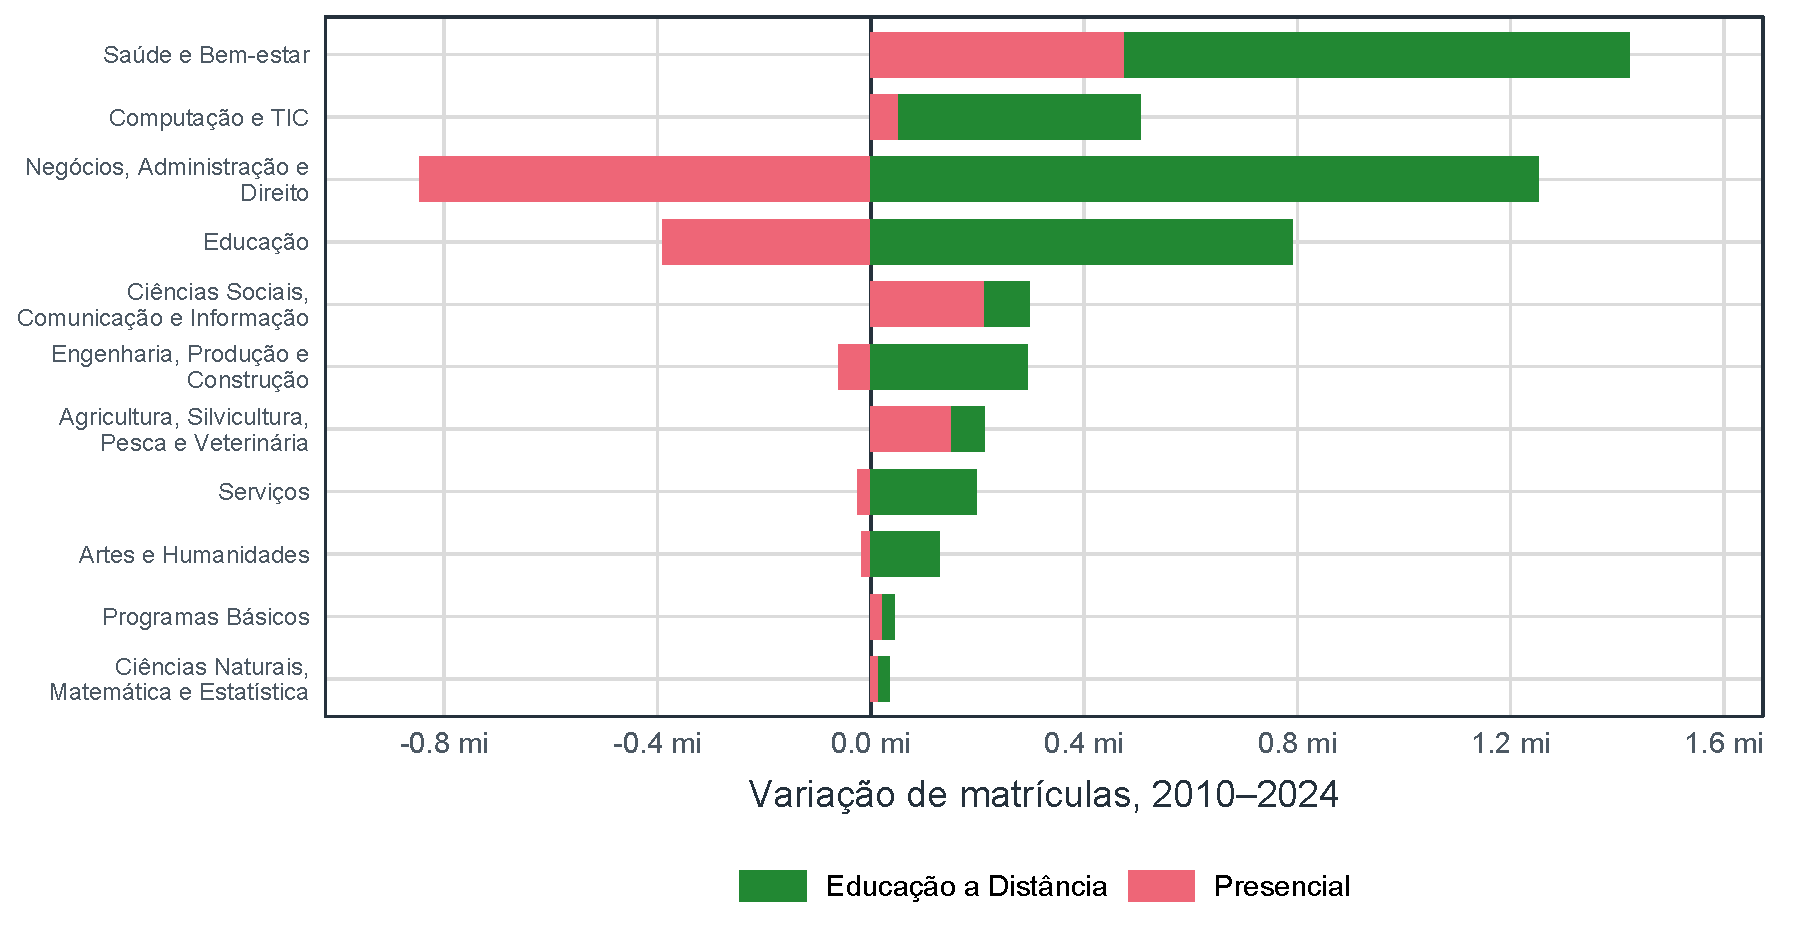
\includegraphics[width=218mm,height=98mm]{apresentacao_files/figure-beamer/plot-b2-1.pdf}
\end{center}

\vfill
\begingroup
\fontsize{8}{10}\selectfont\color{cinzamedio}

Fonte: elaboração própria com base no Censo da Educação Superior e na
ficha B.2.

\endgroup
\end{frame}

\begin{frame}{B.2 --- Principais conclusões}
\protect\phantomsection\label{b.2-principais-conclusuxf5es}
\Rotulo{Saúde e Bem-estar}

\begin{itemize}
\tightlist
\item
  Saúde e Bem-estar respondeu por \textbf{1.4 milhão de novas
  matrículas} entre 2010 e 2024, ou \textbf{37\%} da expansão total;
\item
  Área com o maior crescimento absoluto no ensino presencial e o segundo
  maior no EaD.
\end{itemize}

\Rotulo{Crescimento do EaD com retração do presencial}

\begin{itemize}
\tightlist
\item
  Fenômeno muito forte em Negócios, administração e direito e em
  Educação, mas também presente em outras três áreas;
\end{itemize}

\Rotulo{Crescimento do presencial mais rápido do que EaD}

\begin{itemize}
\tightlist
\item
  Somente Ciências sociais, comunicação e informação e Agricultura,
  silvicultura, pesca e veterinária.
\end{itemize}
\end{frame}

\begin{frame}{B.3}
\protect\phantomsection\label{b.3}
\DescricaoIndicador{Apropriação acumulada do saldo de ingressantes e matrículas por tamanho de mantenedora entre 2010 e 2024}

\Rotulo{Séries}

\begin{itemize}
\tightlist
\item
  Ingressantes e matrículas:

  \begin{itemize}
  \tightlist
  \item
    Total
  \item
    Modalidade de ensino
  \item
    Tamanho de mantenedoras por número de matrículas
  \item
    Turno de ensino
  \item
    Tamanho de mantenedoras por número de matrículas + Modalidade de
    ensino
  \item
    Tamanho de mantenedoras por número de matrículas + Turno de ensino
  \end{itemize}
\end{itemize}
\end{frame}

\begin{frame}{\TituloGrafico{B.3 --- Variação de matrículas por faixas de tamanho de mantenedoras,
modalidade de ensino e turno}}
\protect\phantomsection\label{b.3-variauxe7uxe3o-de-matruxedculas-por-faixas-de-tamanho-de-mantenedoras-modalidade-de-ensino-e-turno}
\begin{center}\begingroup\fontsize{10}{11.5}\selectfont

\begin{tabular}{p{0.57\textwidth}rr}
\toprule
\rowcolor{azulescuro}
\textcolor{white}{\textbf{Grupos}} & \textcolor{white}{\textbf{Variação (milhares)}} & \textcolor{white}{\textbf{Contribuição (\%)}}\\
\midrule
\rowcolor{cinzaclaro}\textbf{Top 5 mantenedoras} & 1,980 & 51\\
\hspace{1em}Educação a Distância & 2,362 & 61\\
\hspace{1em}Diurno & -70 & -2\\
\hspace{1em}Noturno & -311 & -8\\
\rowcolor{cinzaclaro}\textbf{Top 6-10 mantenedoras} & 628 & 16\\
\hspace{1em}Educação a Distância & 401 & 10\\
\hspace{1em}Diurno & 21 & 1\\
\hspace{1em}Noturno & 206 & 5\\
\rowcolor{cinzaclaro}\textbf{Top 11-15 mantenedoras} & 212 & 6\\
\hspace{1em}Educação a Distância & 217 & 6\\
\hspace{1em}Diurno & 5 & 0\\
\hspace{1em}Noturno & -9 & 0\\
\rowcolor{cinzaclaro}\textbf{Top 16-20 mantenedoras} & 118 & 3\\
\hspace{1em}Educação a Distância & 150 & 4\\
\hspace{1em}Diurno & 0 & 0\\
\hspace{1em}Noturno & -32 & -1\\
\rowcolor{cinzaclaro}\textbf{Demais mantenedoras} & 908 & 24\\
\hspace{1em}Educação a Distância & 1,127 & 29\\
\hspace{1em}Diurno & 360 & 9\\
\hspace{1em}Noturno & -579 & -15\\
\rowcolor{cinzaclaro}\textbf{Total} & 3,845 & 100\\
\bottomrule
\end{tabular}
\endgroup\end{center}

\vfill
\begingroup
\fontsize{8}{10}\selectfont\color{cinzamedio}

Fonte: elaboração própria com base nos dados do Censo da Educação
Superior.\newline Nota: as faixas são recalculadas anualmente e
definidas pelo número total de matrículas.

\endgroup
\end{frame}

\begin{frame}{B.3 --- Principais conclusões}
\protect\phantomsection\label{b.3-principais-conclusuxf5es}
\Rotulo{Aumento da concentração em grandes mantenedoras}

\begin{itemize}
\tightlist
\item
  As cinco maiores mantenedoras responderam por \textbf{52\%} do aumento
  das matrículas entre 2010 e 2024.
\item
  Consideradas em conjunto, as vinte maiores concentraram \textbf{76\%}
  da expansão líquida.
\item
  Mais de 1,700 outras mantenedoras responderam pelos 24\% restantes.
\end{itemize}

\Rotulo{EaD cresceu em todas as faixas, mas principalmente entre as maiores}

\begin{itemize}
\tightlist
\item
  Expansão do EaD foi generalizada, embora desigual, com forte ampliação
  de matrículas EaD nas maiores mantenedoras;
\item
  Retração do ensino noturno também foi bastante disseminada;
\item
  Ensino presencial diurno só cresceu entre as ``demais mantenedoras''.
\end{itemize}

\begingroup
\fontsize{11.5}{15.5}\selectfont

\Rotulo{Observações}

A ficha mede a apropriação do crescimento pelas faixas de tamanho. Ela
não identifica, isoladamente, permanência ou substituição de atores no
ranking.

\endgroup
\end{frame}

\begin{frame}[plain]{}
\protect\phantomsection\label{dimensuxe3o-g}
\AberturaSecao{Dimensão G}{Corpo docente}
\end{frame}

\begin{frame}{G.1 *}
\protect\phantomsection\label{g.1}
\DescricaoIndicador{Quantidade de docentes em exercício em tempo integral por modalidade de ensino entre 2010 e 2024}

\Rotulo{Séries}

\begin{itemize}
\tightlist
\item
  Docentes em exercício e Docentes em exercício em tempo integral:

  \begin{itemize}
  \tightlist
  \item
    Total
  \item
    Categoria administrativa
  \item
    Tamanho de mantenedoras por número de matrículas
  \item
    Faixas com percentual de matrículas na educação a distância
  \end{itemize}
\end{itemize}
\end{frame}

\begin{frame}{\TituloGrafico{G.1 --- Docentes em exercício e docentes em exercício em tempo integral}}
\protect\phantomsection\label{g.1-docentes-em-exercuxedcio-e-docentes-em-exercuxedcio-em-tempo-integral}
\begin{center}
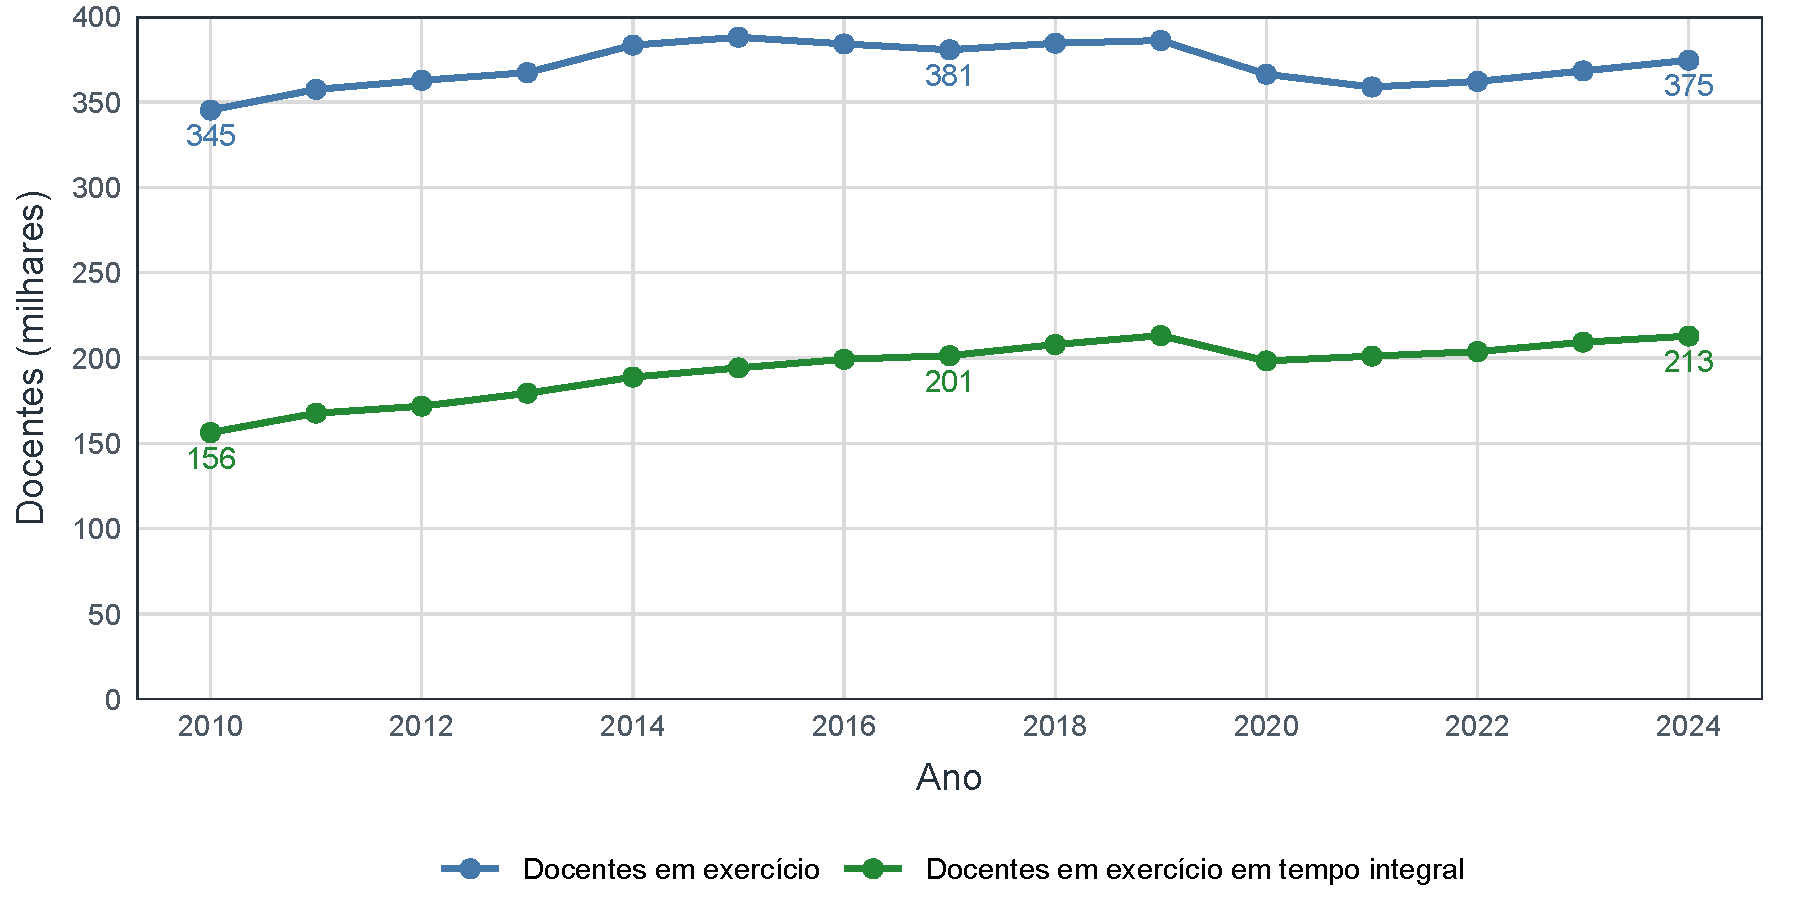
\includegraphics[width=218mm,height=98mm]{apresentacao_files/figure-beamer/plot-g1-total-1.pdf}
\end{center}

\vfill
\begingroup
\fontsize{8}{10}\selectfont\color{cinzamedio}

Fonte: elaboração própria com base no Censo da Educação Superior e na
ficha G.1.

\endgroup
\end{frame}

\begin{frame}{\TituloGrafico{G.1 --- Docentes em exercício por categoria administrativa}}
\protect\phantomsection\label{g.1-docentes-em-exercuxedcio-por-categoria-administrativa}
\begin{center}
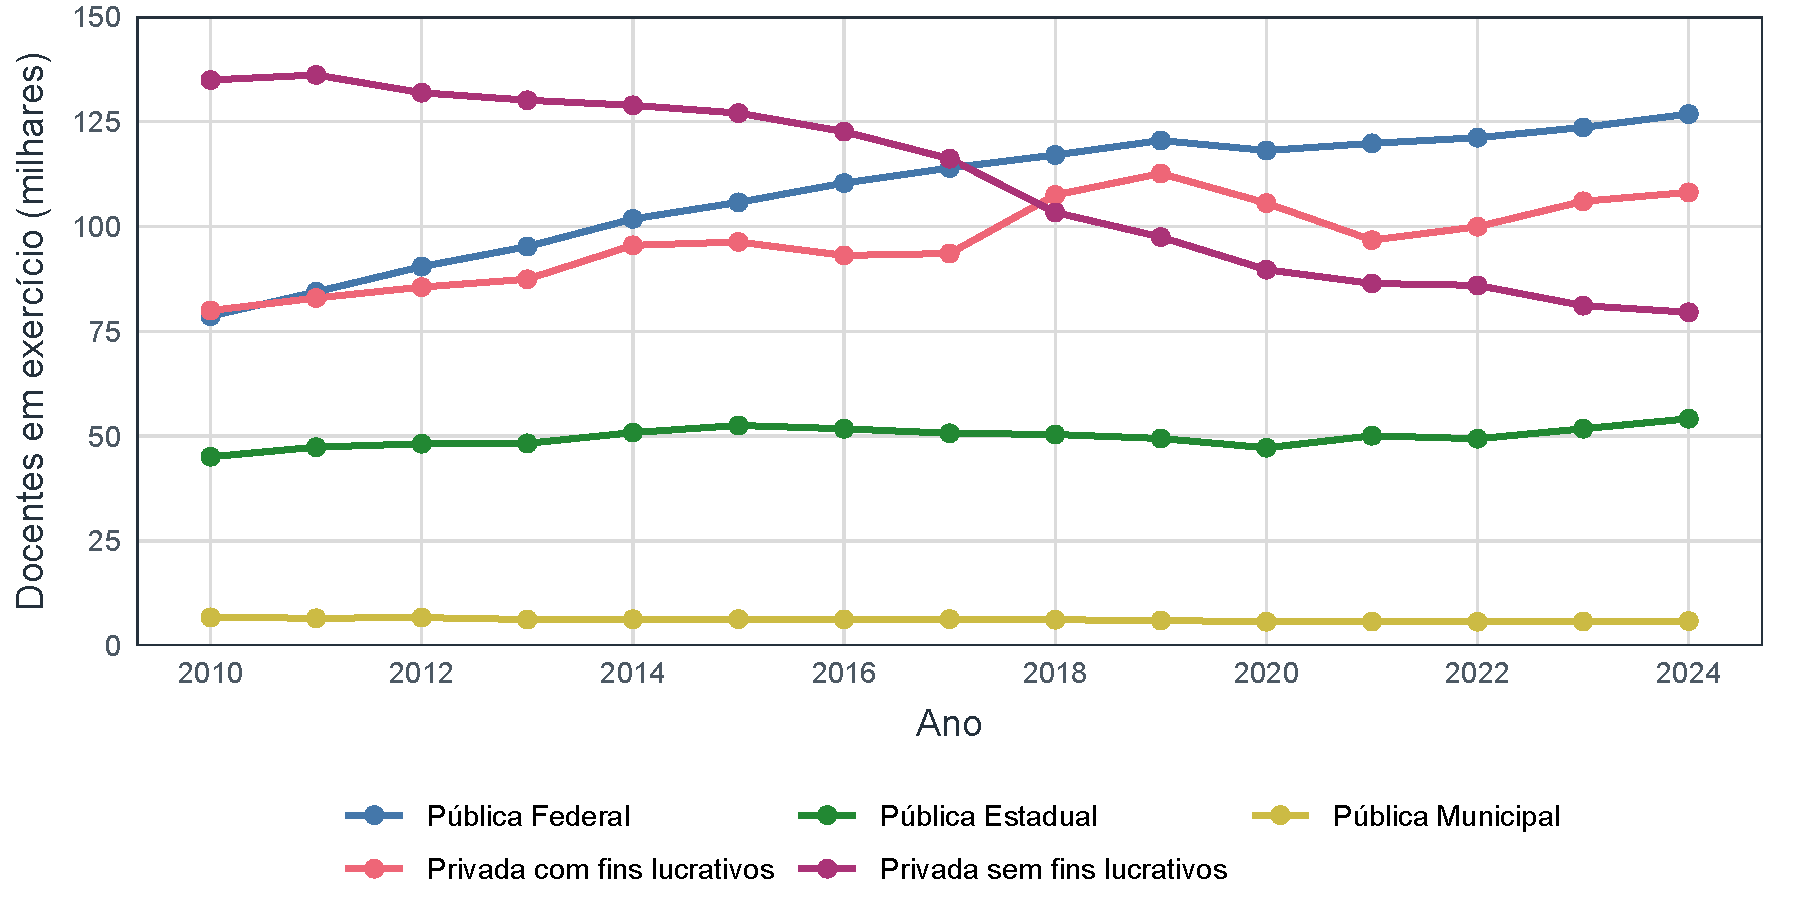
\includegraphics[width=218mm,height=98mm]{apresentacao_files/figure-beamer/plot-g1-categoria-1.pdf}
\end{center}

\vfill
\begingroup
\fontsize{8}{10}\selectfont\color{cinzamedio}

Fonte: elaboração própria com base no Censo da Educação Superior e na
ficha G.1.

\endgroup
\end{frame}

\begin{frame}{G.1 --- Principais conclusões}
\protect\phantomsection\label{g.1-principais-conclusuxf5es}
\Rotulo{Panorama}

\begin{itemize}
\tightlist
\item
  Quantidade de docentes em exercício cresceu \textbf{8\%}, enquanto o
  de docentes em exercício em tempo integral aumentou \textbf{36\%}. O
  percentual em tempo integral foi de 45\% para 57\%.
\item
  O número de matrículas subiu \textbf{60\%}.
\end{itemize}

\Rotulo{Composição por categoria administrativa}

\begin{itemize}
\tightlist
\item
  Quantidade de docentes cresceu \textbf{61\%} nas IES públicas
  federais, \textbf{35\%} nas IES privadas com fins lucrativos e
  \textbf{20\%} nas IES públicas estaduais.
\item
  Houve retração forte nas IES privadas sem fins lucrativos
  (\textbf{41\%}) e modesta nas IES públicas municipais (\textbf{13\%}).
\end{itemize}

\Rotulo{Composição por faixas de tamanho de mantenedoras}

\begin{itemize}
\tightlist
\item
  A quantidade de docentes em exercício nas 20 maiores mantenedoras caiu
  de \textbf{51} para \textbf{40 mil} entre 2010 e 2024
  (\textbf{-22\%}).
\end{itemize}
\end{frame}

\begin{frame}{G.2}
\protect\phantomsection\label{g.2}
\DescricaoIndicador{Titulação do corpo docente (doutor, mestre, especialista) por modalidade de ensino entre 2010 e 2024}

\Rotulo{Séries}

\begin{itemize}
\tightlist
\item
  Docentes em exercício e Docentes em exercício por nível de
  qualificação

  \begin{itemize}
  \tightlist
  \item
    Total
  \item
    Categoria administrativa
  \item
    Tamanho de mantenedoras por número de matrículas
  \item
    Percentual de matrículas na EaD
  \end{itemize}
\end{itemize}
\end{frame}

\begin{frame}{\TituloGrafico{G.2 --- Titulação do corpo docente}}
\protect\phantomsection\label{g.2-titulauxe7uxe3o-do-corpo-docente}
\begin{center}
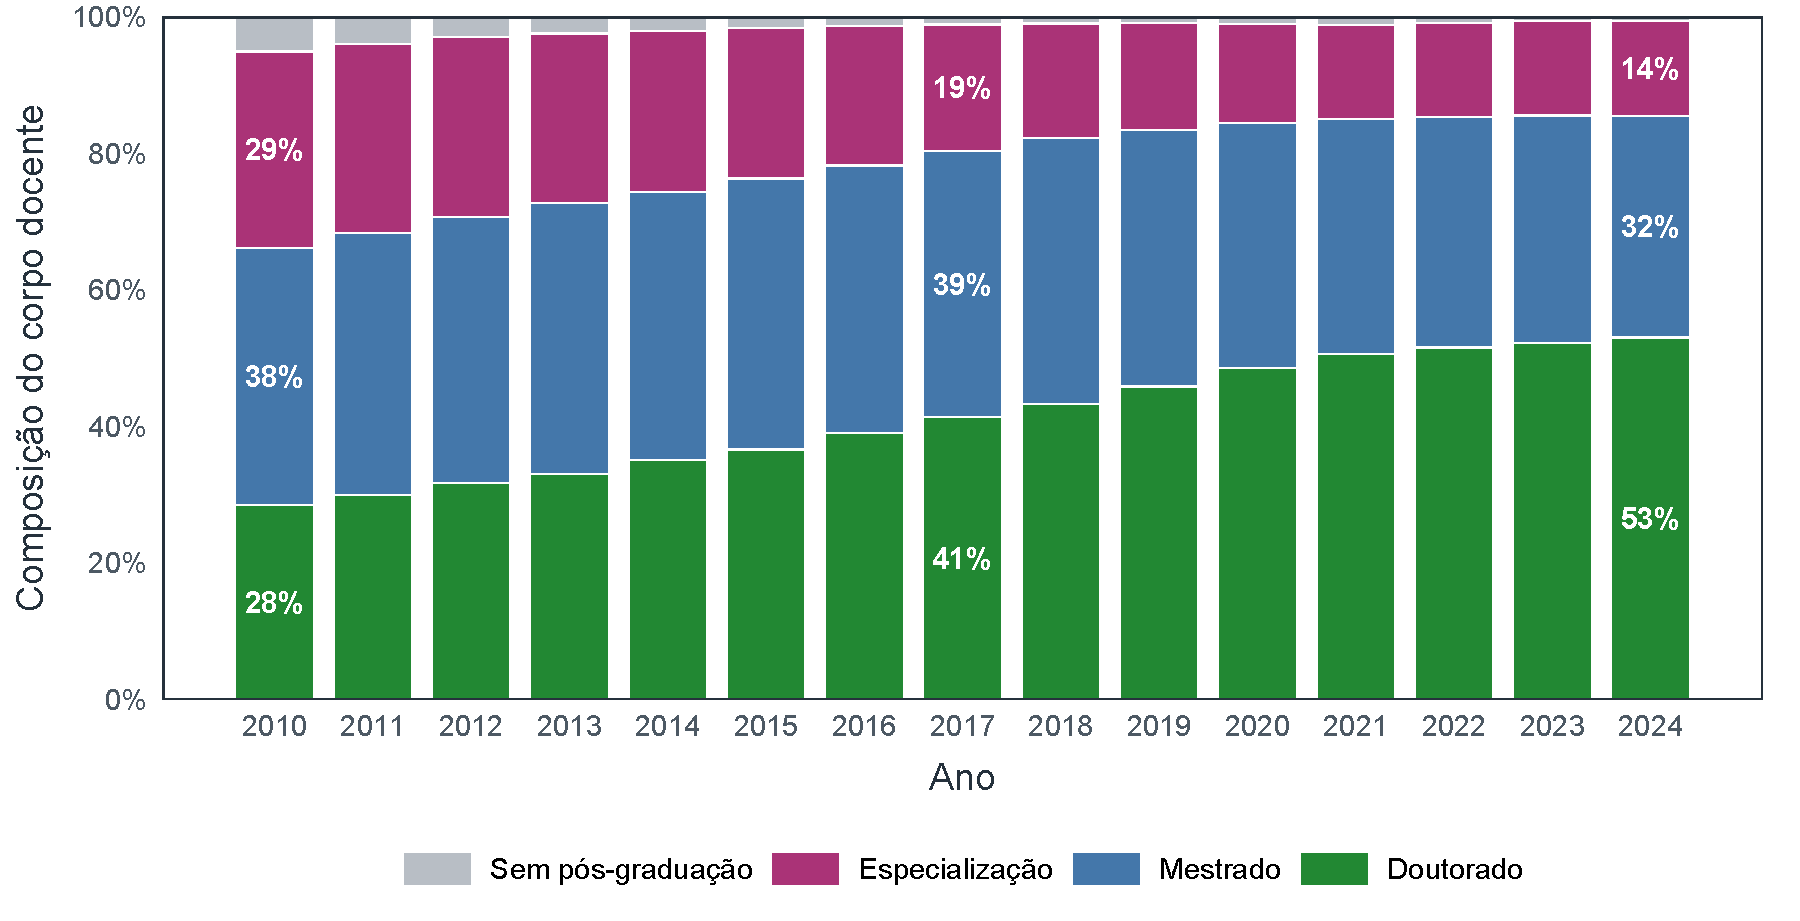
\includegraphics[width=218mm,height=98mm]{apresentacao_files/figure-beamer/plot-g2-1.pdf}
\end{center}

\vfill
\begingroup
\fontsize{8}{10}\selectfont\color{cinzamedio}

Fonte: elaboração própria com base no Censo da Educação Superior e na
ficha G.2.

\endgroup
\end{frame}

\begin{frame}{G.2 --- Principais conclusões}
\protect\phantomsection\label{g.2-principais-conclusuxf5es}
\Rotulo{Titulação mais elevada}

\begin{itemize}
\tightlist
\item
  A participação de docentes com doutorado aumentou de \textbf{28\% para
  53\%} entre 2010 e 2024.
\item
  A parcela com mestrado caiu de 38\% para 33\%, a especialização recuou
  de 29\% para 14\% e docentes sem pós-graduação passaram de 5\% para
  \textbf{1\%}.
\item
  Em números absolutos, os docentes com doutorado aumentaram de 98 mil
  para cerca de 199 mil.
\end{itemize}

\Rotulo{Docentes com doutorado}

\begin{itemize}
\tightlist
\item
  Participação no total cresceu em todas as categorias administrativas,
  mas há ainda há diferença grande entre públicas e privadas. Por
  exemplo:

  \begin{itemize}
  \tightlist
  \item
    IES públicas federais: \textbf{56\%} em 2010 e \textbf{77\%} em
    2024;
  \item
    IES privadas com fins lucrativos: \textbf{11\%} em 2010 e
    \textbf{30\%} em 2024.
  \end{itemize}
\item
  Participação entre as maiores mantenedoras está abaixo da média total.
  Por exemplo:

  \begin{itemize}
  \tightlist
  \item
    Top 5 mantenedoras: \textbf{15\%} em 2010 e \textbf{40\%} em 2024.
  \end{itemize}
\end{itemize}
\end{frame}

\begin{frame}{G.3}
\protect\phantomsection\label{g.3}
\DescricaoIndicador{Regime de trabalho dos docentes (tempo integral, parcial, horário) entre 2010 e 2024}

\Rotulo{Séries}

\begin{itemize}
\tightlist
\item
  Docentes em exercício, em tempo integral e horistas

  \begin{itemize}
  \tightlist
  \item
    Total
  \item
    Categoria administrativa
  \item
    Tamanho de mantenedoras por número de matrículas
  \item
    Percentual de matrículas na EaD
  \end{itemize}
\end{itemize}
\end{frame}

\begin{frame}{\TituloGrafico{G.3 --- Regime de trabalho do corpo docente}}
\protect\phantomsection\label{g.3-regime-de-trabalho-do-corpo-docente}
\begin{center}
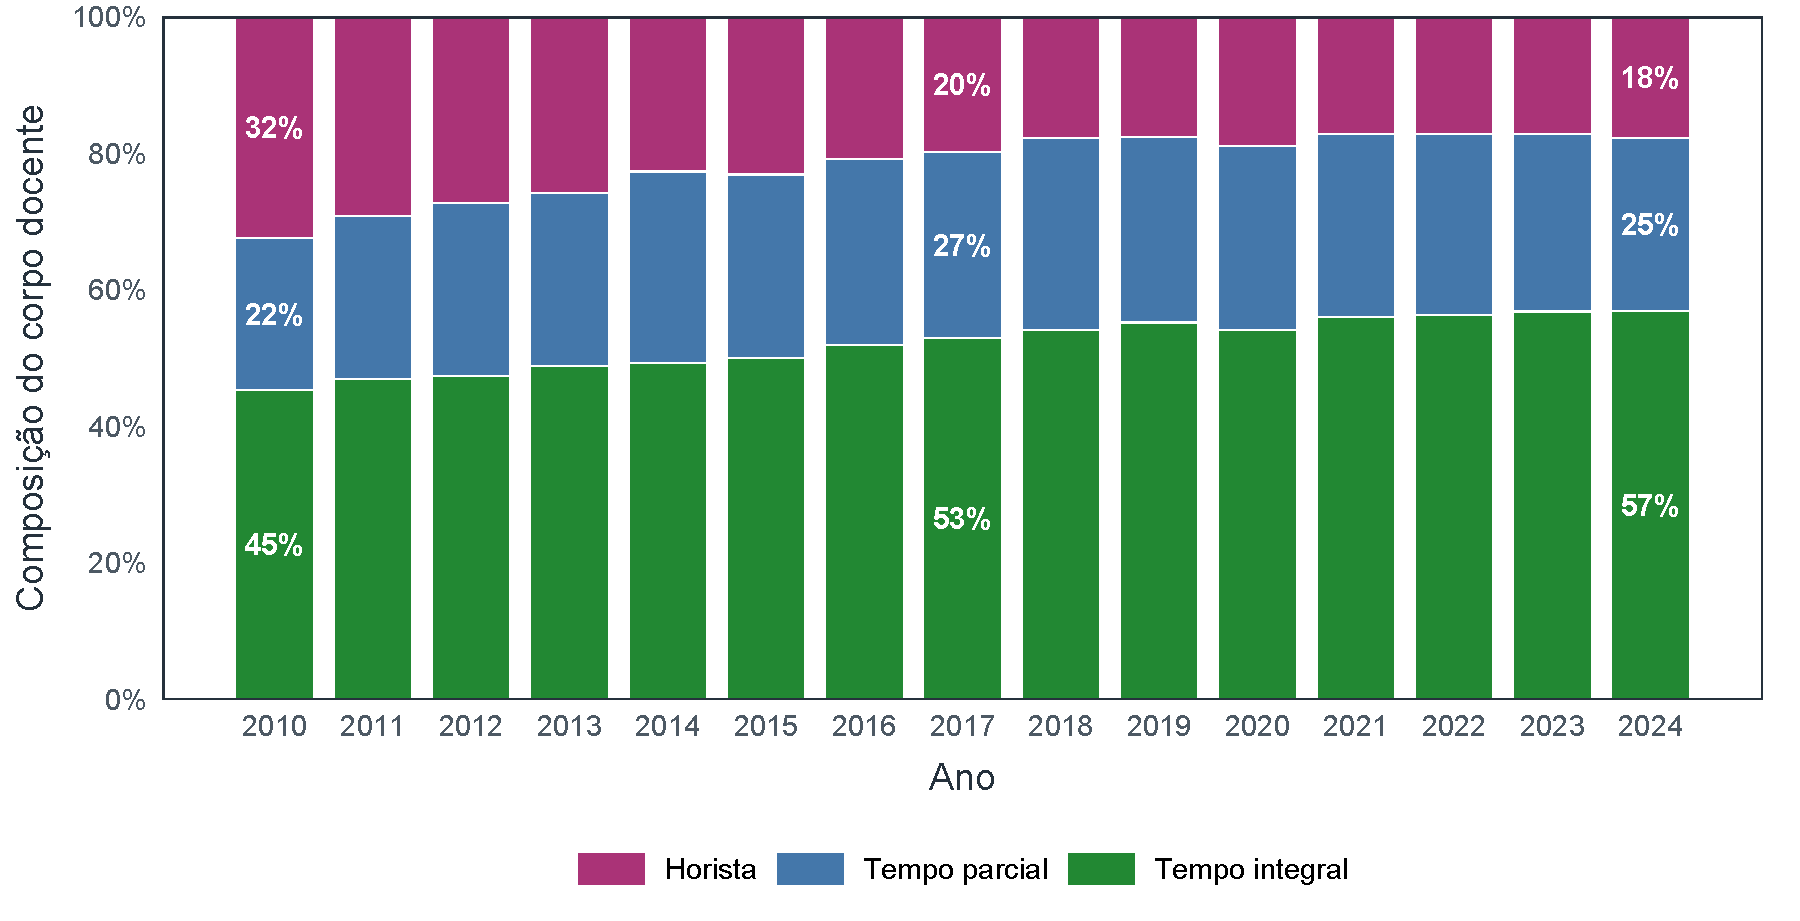
\includegraphics[width=218mm,height=98mm]{apresentacao_files/figure-beamer/plot-g3-1.pdf}
\end{center}

\vfill
\begingroup
\fontsize{8}{10}\selectfont\color{cinzamedio}

Fonte: elaboração própria com base no Censo da Educação Superior e na
ficha G.3.

\endgroup
\end{frame}

\begin{frame}{G.3 --- Principais conclusões}
\protect\phantomsection\label{g.3-principais-conclusuxf5es}
\Rotulo{Panorama}

\begin{itemize}
\tightlist
\item
  Entre 2010 e 2024, a participação do tempo integral subiu de
  \textbf{45\% para 57\%}, enquanto a de horistas caiu de \textbf{32\%
  para 18\%}. O tempo parcial passou de 22\% para 25\%.
\end{itemize}

\Rotulo{Categoria administrativa}

\begin{itemize}
\tightlist
\item
  Em 2010, o tempo integral representava \textbf{90\%} nas IES públicas
  federais e \textbf{21\%} nas privadas com fins lucrativos.
\item
  Em 2024, esses percentuais eram, respectivamente, \textbf{94\%} e
  \textbf{26\%}.
\end{itemize}

\Rotulo{Faixas de tamanho de mantenedoras}

\begin{itemize}
\tightlist
\item
  Nas cinco maiores, a participação do tempo integral recuou de
  \textbf{37\% para 27\%}; nas demais, cresceu de \textbf{44\% para
  59\%}. As faixas são recalculadas a cada ano e não acompanham um
  conjunto fixo de mantenedoras.
\end{itemize}
\end{frame}

\begin{frame}{G.4}
\protect\phantomsection\label{g.4}
\DescricaoIndicador{Relação aluno por docente entre 2010 e 2024}

\Rotulo{Séries}

\begin{itemize}
\tightlist
\item
  Docentes em exercício, em tempo integral e horistas

  \begin{itemize}
  \tightlist
  \item
    Total
  \item
    Categoria administrativa
  \item
    Tamanho de mantenedoras por número de matrículas
  \item
    Percentual de matrículas na EaD
  \end{itemize}
\end{itemize}
\end{frame}

\begin{frame}{\TituloGrafico{G.4 --- Matrículas por docente por categoria administrativa}}
\protect\phantomsection\label{g.4-matruxedculas-por-docente-por-categoria-administrativa}
\begin{center}
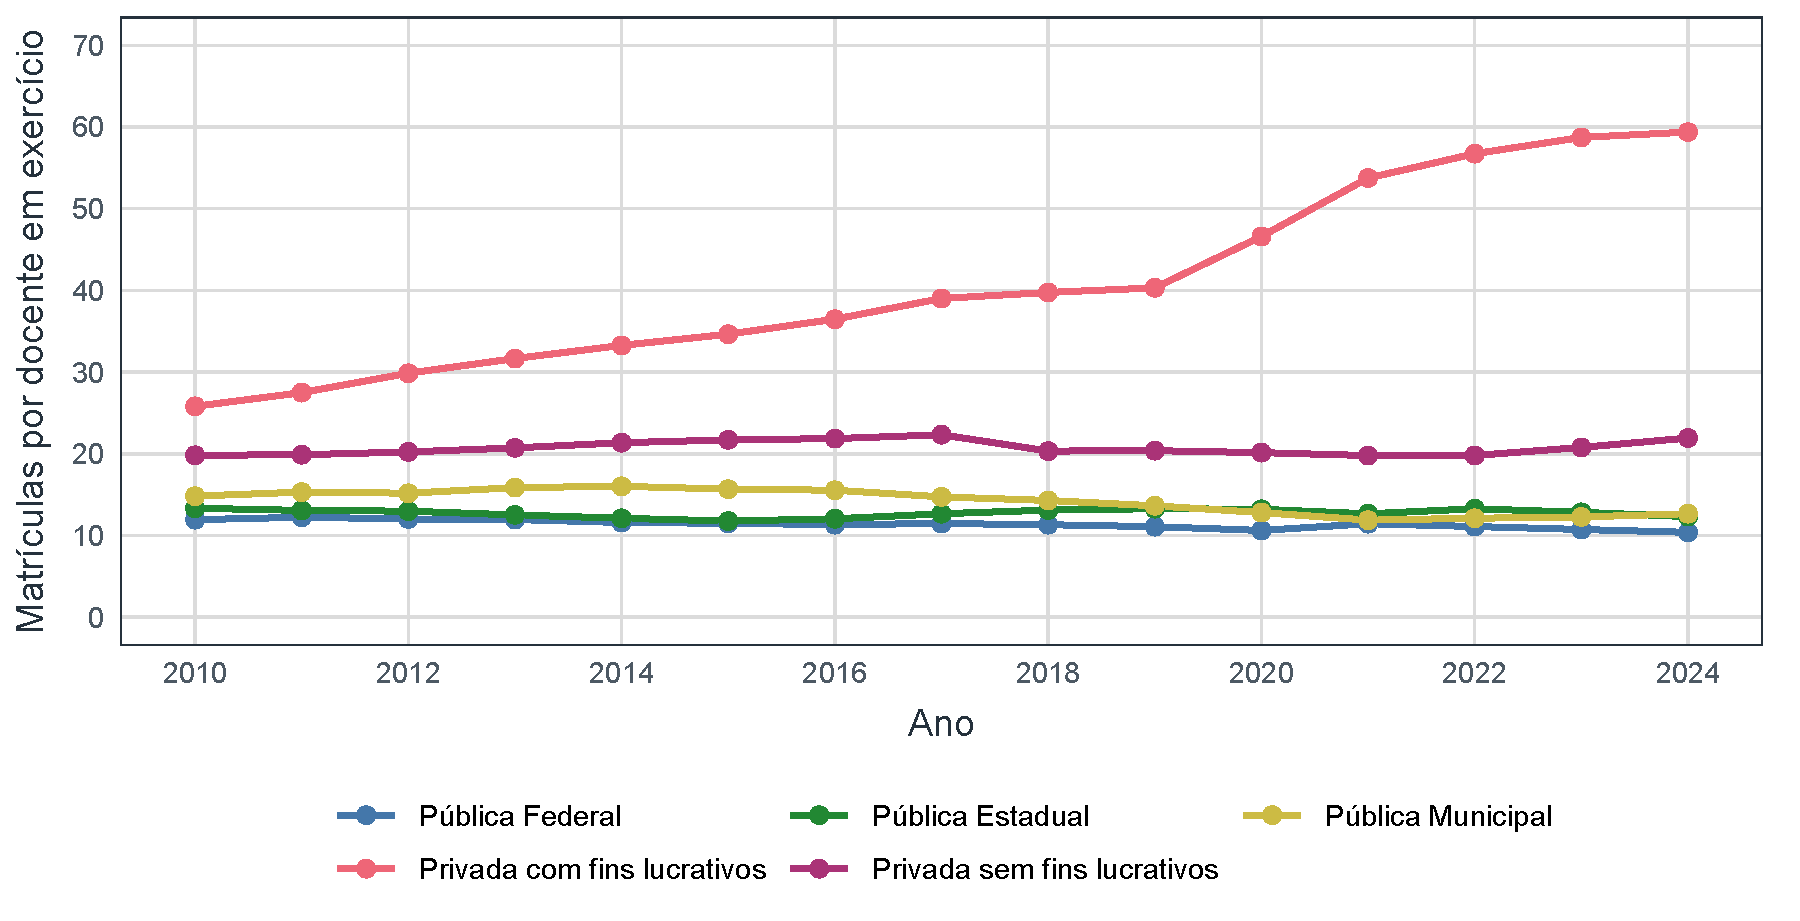
\includegraphics[width=218mm,height=98mm]{apresentacao_files/figure-beamer/plot-g4-categoria-1.pdf}
\end{center}

\vfill
\begingroup
\fontsize{8}{10}\selectfont\color{cinzamedio}

Fonte: elaboração própria com base no Censo da Educação Superior e na
ficha G.4.

\endgroup
\end{frame}

\begin{frame}{\TituloGrafico{G.4 --- Matrículas por docente por tamanho da mantenedora}}
\protect\phantomsection\label{g.4-matruxedculas-por-docente-por-tamanho-da-mantenedora}
\begin{center}
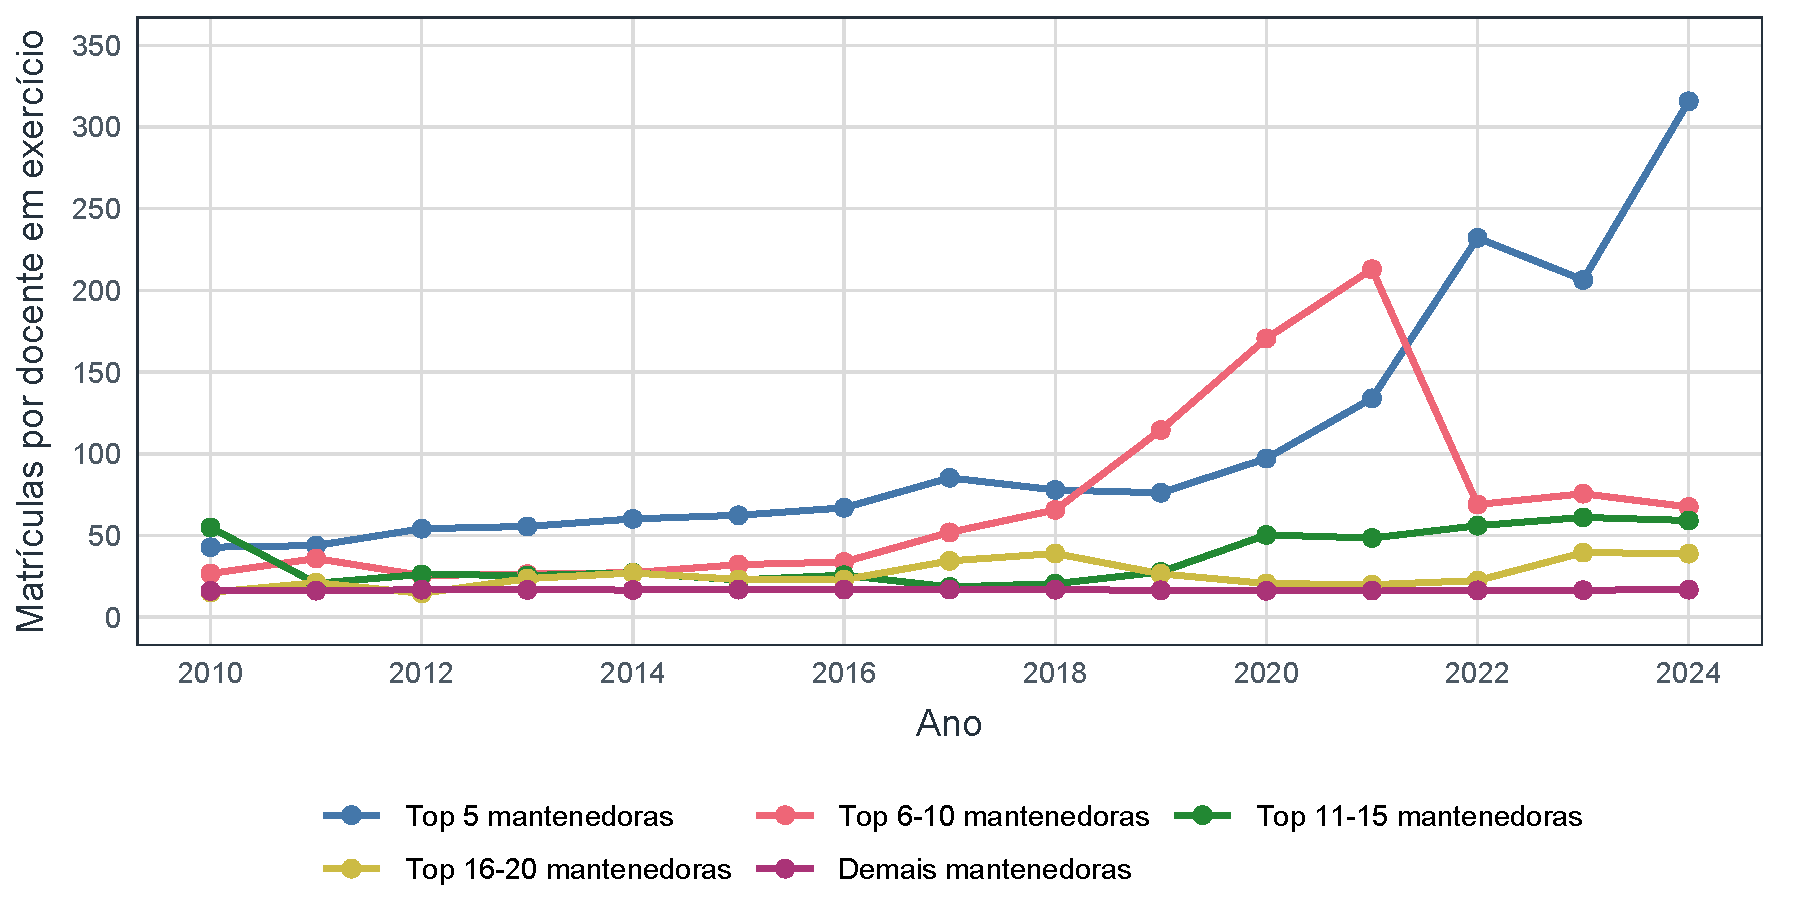
\includegraphics[width=218mm,height=98mm]{apresentacao_files/figure-beamer/plot-g4-tamanho-1.pdf}
\end{center}

\vfill
\begingroup
\fontsize{8}{10}\selectfont\color{cinzamedio}

Fonte: elaboração própria com base no Censo da Educação Superior e na
ficha G.4. As faixas de tamanho são recalculadas a cada ano.

\endgroup
\end{frame}

\begin{frame}{G.4 --- Principais conclusões}
\protect\phantomsection\label{g.4-principais-conclusuxf5es}
\Rotulo{Panorama}

\begin{itemize}
\tightlist
\item
  No conjunto do sistema, a razão passou de \textbf{18.5 para 27.3
  matrículas por docente} entre 2010 e 2024. O indicador compara volumes
  agregados por IES; não mede o tamanho das turmas.
\end{itemize}

\Rotulo{Categoria administrativa}

\begin{itemize}
\tightlist
\item
  Nas IES privadas com fins lucrativos, a razão subiu de \textbf{25.8
  para 59.4}. Nas públicas, ficou entre \textbf{10.4 e 12.7} matrículas
  por docente em 2024.
\end{itemize}

\Rotulo{Faixas de tamanho de mantenedoras}

\begin{itemize}
\tightlist
\item
  Nas cinco maiores, a razão passou de \textbf{42.8 para 315.8}; nas
  demais, de \textbf{16.1 para 16.8}. As faixas são recalculadas a cada
  ano e não representam um conjunto fixo de mantenedoras.
\end{itemize}
\end{frame}




\end{document}
